\section{Proposed Methodology}\label{sec:method}

This section delineates the core algorithmic components of the Vecna multimodal retrieval framework. We first formalize the query expansion mechanism governed by strict hallucination boundaries (\S\ref{sec:hyde}). Subsequently, we introduce our hybrid dense-sparse multimodal fusion strategy (\S\ref{sec:fusion}) and the dynamic programming formulation for temporal sequence alignment (\S\ref{sec:temporal}). Finally, we present our scene-aware segment diversification algorithm (\S\ref{sec:diversify}) and the cryptographic provenance architecture ensuring data integrity (\S\ref{sec:provenance}).

\subsection{Multi-Aspect Factual HyDE with Zero-Speculation Boundaries}\label{sec:hyde}

To bridge the modality gap between terse user queries and the rich semantic space of multimodal embeddings, we define an expansion function utilizing a Large Language Model (LLM):
\begin{equation}
\mathcal{F}_{\text{LLM}}(q_{\text{raw}}) \rightarrow \Psi = \langle q_{\text{corr}}, q_{\text{hyde}}^{\text{vi}}, q_{\text{en}}, q_{\text{para}}, \mathbf{K} \rangle
\end{equation}
The output tuple $\Psi$ encapsulates multiple facets of the information need:
\begin{itemize}
    \item $q_{\text{corr}}$: The orthographically corrected query, preserving the source language semantics and diacritics.
    \item $q_{\text{hyde}}^{\text{vi}}$: A simulated visual keyframe description in Vietnamese, strictly constrained to delineating the primary subject, action, camera perspective, and lighting conditions.
    \item $q_{\text{en}}$: A concise English caption (15--35 words) structurally analogous to LAION and WebLI datasets, optimized for alignment with OpenCLIP and SigLIP dual-encoder spaces.
    \item $q_{\text{para}}$: A set of semantic synonyms within the source language to broaden the dense retrieval manifold.
    \item $\mathbf{K}$: A tuple of sparse and dense keywords for exact lexical matching and inverted index querying.
\end{itemize}

Crucially, $\mathcal{F}_{\text{LLM}}$ is governed by the \textit{Zero-Speculation Constraint}. We formalize this constraint as a rejection sampling boundary that strictly prohibits the generation of ungrounded proper nouns, dates, or numerals that do not exist within the token set of $q_{\text{raw}}$. This prevents semantic drift and spurious correlations. To ensure real-time responsiveness, $\mathcal{F}_{\text{LLM}}$ is wrapped in a Least Recently Used (LRU) cache (capacity $N=20$), yielding a 0ms overhead for repetitive query formulations.

\subsection{Multi-Modal Hybrid Fusion and Exact Phrase Matching}\label{sec:fusion}

To construct the unified relevance manifold, we employ a weighted multi-modal fusion strategy. For a given candidate keyframe $f$, dense visual similarity is computed via cosine similarity between $L_2$-normalized query embedding $\mathbf{e}_q$ and frame embedding $\mathbf{e}_f$:
\begin{equation}
S_{\text{vis}}(q, f) = \frac{\mathbf{e}_q \cdot \mathbf{e}_f}{\|\mathbf{e}_q\| \|\mathbf{e}_f\|}
\end{equation}
The composite multi-modal retrieval score across visual, optical text, and speech channels is evaluated as:
\begin{equation}
S_{\text{total}}(f) = w_{\text{vis}} \tilde{S}_{\text{vis}}(f) + w_{\text{ocr}} \tilde{S}_{\text{ocr}}(f) + w_{\text{asr}} \tilde{S}_{\text{asr}}(f)
\end{equation}
where $w_{\text{vis}} = 1.0 - w_{\text{ocr}} - w_{\text{asr}}$, and $\tilde{S}_{(\cdot)}(f) = S_{(\cdot)}(f) / \max S_{(\cdot)}$ represents max-scale normalized scores. Here, $\tilde{S}_{\text{vis}}$ denotes the score from the active visual model ensemble (OpenCLIP, SigLIP, and/or Qwen3-VL). For textual modalities $m \in \{\text{ocr}, \text{asr}\}$, score $\tilde{S}_m$ is a convex combination of dense BGE-M3 semantic similarity and sparse BM25 lexical alignment:
\begin{equation}
\tilde{S}_m(f) = (1 - \alpha_m) \cdot \tilde{S}_{\text{dense}}^{(m)}(f) + \alpha_m \cdot \tilde{S}_{\text{sparse}}^{(m)}(f)
\end{equation}

\textbf{Exact-Phrase Boundary Verifier}: Quoted search terms (e.g., \texttt{"VTV1"} or literal banners) trigger a regular expression filter with diacritic insensitivity and elastic word boundaries:
\begin{equation}
R_{\text{exact}} = \text{RegEx}\big((?<!\backslash w) + \text{phrase} + (?!\backslash w)\big)
\end{equation}
Matching frames receive an empirical $1.5\times$ score boost, while non-matching frames are strictly eliminated from the candidate pool to preserve high precision.

\textbf{Dynamic Candidate Replenishment}: When negative video filtering (e.g., \texttt{[!video:L18\_V005]}) excludes non-target candidates, naive post-filtering frequently depletes pagination views. To maintain full result sets, Vecna implements an adaptive replenishment loop: initial candidate retrieval begins at $\max(300, (\text{offset} + \text{limit}) \times 3)$ and doubles dynamically until at least $(\text{offset} + \text{limit})$ valid candidate frames populate the view:
\begin{equation}
K^{(t+1)} = \min\big(D_{\max}, 2 \cdot K^{(t)}\big)
\end{equation}

\subsection{Temporal Multi-Step Sequence Alignment via Dynamic Programming}\label{sec:temporal}

For multi-event chronological queries $Q = \langle q_1, \dots, q_M \rangle$ delimited by \texttt{/} or \texttt{;}, candidate pools $\mathcal{F}_i$ are retrieved for each step up to $k = \text{temporal\_k}$. The dynamic programming algorithm determines the optimal chronological sequence score $D(i, f)$ for candidate frame $f \in \mathcal{F}_i$:
\begin{equation}
D(i, f) = S(q_i, f) + \max_{f' \in \mathcal{F}_{i-1}} \Big\{ D(i-1, f') \;\Big|\; 0 < t(f) - t(f') \le \Delta t_{\max} \Big\}
\end{equation}
where $\Delta t_{\max} = 1000$ frames serves as the temporal horizon.

To solve this efficiently, we propose a Two-Pointer Sliding-Window Temporal Dynamic Programming algorithm (Algorithm~\ref{alg:dp}, illustrated in Figure~\ref{fig:temporal_dp}). 

\begin{figure}[t]
    \centering
    \resizebox{\columnwidth}{!}{%
    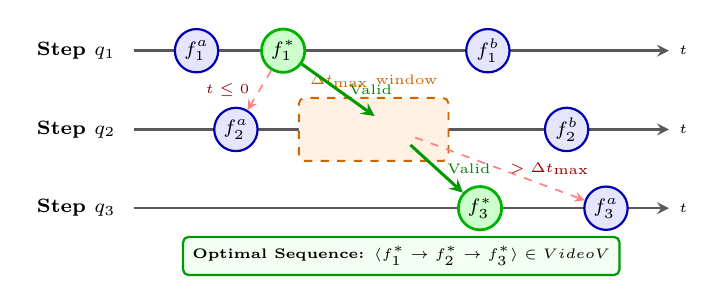
\begin{tikzpicture}[
        >=stealth, thick, font=\sffamily\scriptsize,
        timeline/.style={->, line width=0.9pt, draw=gray!70!black},
        cand/.style={circle, draw=blue!70!black, fill=blue!10, inner sep=1pt, minimum size=5.5mm, font=\scriptsize\bfseries},
        candactive/.style={circle, draw=green!70!black, fill=green!20, inner sep=1pt, minimum size=5.5mm, font=\scriptsize\bfseries, line width=1.0pt},
        window/.style={draw=orange!80!black, fill=orange!10, rounded corners=2pt, dashed, line width=0.7pt},
        conn/.style={->, draw=green!60!black, line width=1.1pt},
        pruned/.style={->, draw=red!50, dashed, line width=0.6pt}
    ]
    % Timelines for sub-queries
    \draw[timeline] (0, 2.0) -- (6.8, 2.0) node[right, font=\tiny] {$t$};
    \node[font=\bfseries\scriptsize, anchor=east] at (-0.1, 2.0) {Step $q_1$};
    
    \draw[timeline] (0, 1.0) -- (6.8, 1.0) node[right, font=\tiny] {$t$};
    \node[font=\bfseries\scriptsize, anchor=east] at (-0.1, 1.0) {Step $q_2$};
    
    \draw[timeline] (0, 0.0) -- (6.8, 0.0) node[right, font=\tiny] {$t$};
    \node[font=\bfseries\scriptsize, anchor=east] at (-0.1, 0.0) {Step $q_3$};

    % Candidates on q1
    \node[cand] (c11) at (0.8, 2.0) {$f_1^a$};
    \node[candactive] (c12) at (1.9, 2.0) {$f_1^*$};
    \node[cand] (c13) at (4.5, 2.0) {$f_1^b$};

    % Candidates on q2
    \node[cand] (c21) at (1.3, 1.0) {$f_2^a$};
    \node[candactive] (c22) at (3.3, 1.0) {$f_2^*$};
    \node[cand] (c23) at (5.5, 1.0) {$f_2^b$};

    % Candidates on q3
    \node[candactive] (c31) at (4.4, 0.0) {$f_3^*$};
    \node[cand] (c32) at (6.0, 0.0) {$f_3^a$};

    % Sliding window around c12
    \draw[window] (2.1, 0.6) rectangle (4.0, 1.4);
    \node[font=\tiny, text=orange!80!black, anchor=south] at (3.05, 1.4) {$\Delta t_{\max}$ window};

    % Transitions
    \draw[conn] (c12) -- (c22) node[midway, right, font=\tiny, text=green!50!black] {Valid};
    \draw[conn] (c22) -- (c31) node[midway, right, font=\tiny, text=green!50!black] {Valid};
    \draw[pruned] (c12) -- (c21) node[midway, left, font=\tiny, text=red!60!black] {$t \le 0$};
    \draw[pruned] (c22) -- (c32) node[midway, right, font=\tiny, text=red!60!black] {$> \Delta t_{\max}$};

    % Optimal sequence badge
    \node[draw=green!60!black, fill=green!5, rounded corners=2pt, font=\tiny\bfseries, anchor=north] at (3.4, -0.35) {Optimal Sequence: $\langle f_1^* \rightarrow f_2^* \rightarrow f_3^* \rangle \in \text{Video } V$};
    \end{tikzpicture}%
    }
    \vspace{-2mm}
    \Description{Two-pointer sliding-window temporal sequence alignment algorithm schematic.}
    \caption{Two-pointer sliding-window temporal sequence alignment. For multi-step chronological queries $\langle q_1, q_2, q_3 \rangle$, candidate transitions are constrained within the forward temporal window $(0, \Delta t_{\max}]$, eliminating non-monotonic and out-of-bounds candidates in $\mathcal{O}(|C_i| + |B|)$ amortized time.}
    \label{fig:temporal_dp}
    \vspace{-2mm}
\end{figure}

\begin{algorithm}[t]
\caption{Two-Pointer Sliding-Window Temporal DP}
\label{alg:dp}
\textbf{Input}: Sequence of candidate sets $C_1, \dots, C_M$, max temporal gap $\Delta t_{\max}$, queue size $K_{\text{queue}}$ \\
\textbf{Output}: Top-$K_{\text{queue}}$ chronological tuples
\begin{algorithmic}[1]
\STATE Initialize buffer $B \leftarrow \text{Top-}K_{\text{queue}}(C_M)$
\FOR{$i = M-1$ \textbf{downto} $1$}
    \STATE Sort $C_i$ and $B$ lexicographically by (video\_id, timestamp)
    \STATE Initialize $T_{\text{next}} \leftarrow \emptyset$
    \STATE Initialize two pointers $l \leftarrow 0, r \leftarrow 0$
    \FOR{\textbf{each} $c \in C_i$}
        \STATE Advance $l$ to first $b \in B$ s.t. $b.\text{video} = c.\text{video}$ and $b.\text{time} > c.\text{time}$
        \STATE Advance $r$ to last $b \in B$ s.t. $b.\text{time} \le c.\text{time} + \Delta t_{\max}$
        \FOR{\textbf{each} valid successor $b \in B[l:r]$}
            \STATE Accumulate fusion score: $S_{\text{new}} \leftarrow c.\text{score} + b.\text{score}$
            \STATE Concatenate timeline: $seq_{\text{new}} \leftarrow \langle c \rangle \oplus b.\text{seq}$
            \STATE $T_{\text{next}} \leftarrow T_{\text{next}} \cup \{(S_{\text{new}}, seq_{\text{new}})\}$
        \ENDFOR
    \ENDFOR
    \STATE $B \leftarrow \text{Top-}K_{\text{queue}}(T_{\text{next}})$
\ENDFOR
\RETURN $B$
\end{algorithmic}
\end{algorithm}

Because the candidate sets $C_i$ and the intermediate buffer $B$ are sorted, the two pointers sweep monotonically across the timeline. The amortized time complexity of this step is strictly $\mathcal{O}(\sum_{i=1}^{M-1} (|C_i| + |B|))$. Importantly, the algorithm preserves the per-step intermediate score vectors $S_{\text{hybrid}}(f_j)$, providing crucial interpretability for the final aligned sequence.

\subsection{Semantic Scene Smoothing and Segment-Level Diversification}\label{sec:diversify}

To prevent top ranks from being saturated by visually identical consecutive frames, the framework computes an offline Segment Clustering map (\texttt{build\_segment\_map.py}):
\begin{enumerate}[label=\arabic*.]
    \item Compute adjacent-keyframe cosine similarities $C_t = \cos(\mathbf{e}_t, \mathbf{e}_{t+1})$ across keyframes of each video.
    \item Apply temporal moving-average smoothing across a symmetric window $K = 5$:
    \begin{equation}
    \bar{C}_t = \frac{1}{K} \sum_{i=-2}^{2} C_{t+i}
    \end{equation}
    \item Determine scene transition boundaries by cutting at the lower 5\% quantile ($Q = 0.05$) bounded by adaptive floors $\{0.35, 0.55, 0.75\}$ to achieve $\approx 1$ segment per 60 seconds of video footage.
    \item During online search, the segment diversification operator $\mathcal{D}(R)$ retains only the highest-scoring keyframe per segment across the top candidate pool, maximizing visual variety:
    \begin{equation}
    \mathcal{D}(R) = \{r_i \in R \mid \forall j < i, \text{SegID}(r_i) \neq \text{SegID}(r_j)\}
    \end{equation}
\end{enumerate}

\subsection{Cryptographic Data Provenance Architecture}\label{sec:provenance}

Ensuring the immutability and precise attribution of both raw media and derived features is paramount for reproducible multimedia retrieval. We design a sidecar-based cryptographic provenance architecture. The metadata hierarchy is strictly delineated:
\begin{itemize}
    \item \texttt{sources/\textless video\textgreater.json}: Contains the SHA-256 fixity checksum of the original media file, alongside canonical codec parameters and rational frame rates (FPS).
    \item \texttt{keyframes/\textless video\textgreater.json}: Logs the generation ID of the keyframe selection protocol and the cryptographic fingerprint of the extraction algorithm.
    \item \texttt{evidence/\textless video\textgreater/\textless feature\textgreater/\textless run\textgreater.json}: Stores high-fidelity derived evidence. This includes exact PaddleOCR bounding box coordinates with VietOCR recognition confidence scores, WhisperX native temporal intervals, and the non-linear projection mapping back to the canonical keyframe timeline.
\end{itemize}
A fundamental axiom of this architecture is that historical data provenance remains structurally immutable; it is `unknown' if missing and is never retrospectively backfilled. The identity of any extracted evidence is intrinsically content-sensitive and inextricably bound to its source generation run.
